\subsection{函子性质}

命题 6. 设 G、H 为李群，\(\phi\) 为 G 到 H 的态射。对 \(t, t'\)（\(\mathcal{T}^{(\infty)}(G)\) 中的元素），有 \(\phi_{*}(t * t') = \phi_{*}(t) * \phi_{*}(t')\)。

考虑图

\[
\begin{array}{c} \mathrm{G} \times \mathrm{G} \xrightarrow {m} \mathrm{G} \\ \phi \times \phi \Biggl \downarrow \\ \mathrm{H} \times \mathrm{H} \xrightarrow {n} \mathrm{H} \end{array}
\]

其中 \(m(g, g') = gg'\)，\(n(h, h') = hh'\)。这个图是交换的。因而

\[
\begin{array}{r l} \phi_ {*} (t * t ^ {\prime}) & = \phi_ {*} (m _ {*} (t \otimes t ^ {\prime})) = n _ {*} ((\phi \times \phi) _ {*} (t \otimes t ^ {\prime})) \\ & = n _ {*} (\phi_ {*} (t) \otimes \phi_ {*} (t ^ {\prime})) = \phi_ {*} (t) * \phi_ {*} (t ^ {\prime}). \end{array}
\]

李群 G 与 \(G^{\vee}\) 有相同的底层流形，因而向量空间 \(\mathcal{T}^{(\infty)}(G)\) 与 \(\mathcal{T}^{(\infty)}(G^{\vee})\) 相同。设 \(\theta\) 为映射 \(g \mapsto g^{-1}\)，它是李群 G 到李群 \(G^{\vee}\) 的同构。于是 \(\theta^{*}\) 是向量空间 \(\mathcal{T}^{(\infty)}(G)\) 的一个自同构，我们把它记作 \(t \mapsto t^{\vee}\)。这时 \((\varepsilon_{g})^{\vee} = \varepsilon_{g^{-1}}\)。若 \(t \in T_{e}(G)\)，则

\[
t ^ {\vee} = - t \quad (\S 2, \text { Proposition   2 }).\tag{2}
\]

例。设 G 是由完备可赋范空间 E 定义的李群。于是 U(G) 与 TS(E) 认同，且 \(\theta_{*}\) 在 U(G) 上的限制与 TS(T \(_{e}(\theta)\) ) 认同 (Differentiable and Analytic Manifolds, R, 13.2.4)。因此，若 \(t \in \mathsf{TS}^{s}(E)\)，则 \(t^{\vee} = (-1)^{s}t\)。

命题 7. 设 G 为李群。设 \(t, t'\) 属于 \(\mathcal{T}^{(\infty)}(G)\)。

\begin{enumerate}
\def\labelenumi{(\roman{enumi})}
\item
  乘积 \(t * t'\)（相对于 \(G^{\vee}\) 算得）等于乘积 \(t' * t\)（相对于 \(G\) 算得）。
\item
  \((t*t')^{\vee}=t'^{\vee}*t^{\vee}\)。
\end{enumerate}

考虑下图

\pandocbounded{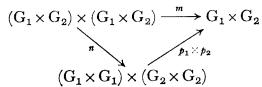
\includegraphics[keepaspectratio]{images/part002_baaabc67.jpg}}

其中 \(s(g, g') = (g', g)\)，\(m(g, g') = gg'\)，\(n(g, g') = g'g\)，这里 \(g\)、\(g'\) 取遍 \(G\)。这个图是交换的。因而 \(n_*(t \otimes t') = m_*(s_*(t \otimes t')) = m_*(t' \otimes t)\)。这个等式恰好就是 (i)。断言 (ii) 由 (i) 与命题 6 得出。

命题 8. 设 G、H 为李群，\(\phi\) 为 G 到 H 的态射。若 \(t \in \mathcal{T}^{(\infty)}(G)\)，则 \(\phi_{*}(t^{\vee}) = (\phi_{*}(t))^{\vee}\)。

设 \(\theta\)（相应地 \(\theta'\)）为 G 到 G（相应地 H 到 H）的映射 \(g \mapsto g^{-1}\)。于是 \(\phi \circ \theta = \theta' \circ \phi\)，从而 \(\phi_*(\theta_*(t)) = \theta'_*(\phi_*(t))\)。

命题 9. 设 \(\mathrm{G}_1, \cdots, \mathrm{G}_n\) 为李群，\(\mathrm{G} = \mathrm{G}_1 \times \cdots \times \mathrm{G}_n\)。若向量空间 \(\mathcal{T}^{(\infty)}(\mathrm{G})\) 与 \(\mathcal{T}^{(\infty)}(\mathrm{G}_1) \otimes \cdots \otimes \mathcal{T}^{(\infty)}(\mathrm{G}_n)\) 典范地认同，则代数 \(\mathcal{T}^{(\infty)}(\mathrm{G})\) 是诸代数 \(\mathcal{T}^{(\infty)}(\mathrm{G}_1), \ldots, \mathcal{T}^{(\infty)}(\mathrm{G}_n)\) 的张量积。若 \(t_i \in \mathcal{T}^{(\infty)}(\mathrm{G}_i)\)（\(i = 1, \ldots, n\)），则

\[
\left(t _ {1} \otimes \dots \otimes t _ {n}\right) ^ {\vee} = t _ {1} ^ {\vee} \otimes \dots \otimes t _ {n} ^ {\vee}.
\]

只需考虑 \(n = 2\) 的情形。设 \(t_1, t_1'\) 属于 \(\mathcal{T}^{(\infty)}(\mathrm{G}_1)\)，\(t_2, t_2'\) 属于 \(\mathcal{T}^{(\infty)}(\mathrm{G}_2)\)。我们需要证明 \((t_1 \otimes t_2) * (t_1' \otimes t_2') = (t_1 * t_1') \otimes (t_2 * t_2')\) 以及 \((t_1 \otimes t_2)^{\vee} = t_1^{\vee} \otimes t_2^{\vee}\)。考虑图

\pandocbounded{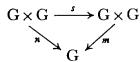
\includegraphics[keepaspectratio]{images/part002_69e6a490.jpg}}

其中 \(m((x_1, x_2), (x_1', x_2')) = (x_1x_1', x_2x_2')\)，

\[
n ((x _ {1}, x _ {2}), (x _ {1} ^ {\prime}, x _ {2} ^ {\prime})) = ((x _ {1}, x _ {1} ^ {\prime}), (x _ {2}, x _ {2} ^ {\prime})),
\]

\(p_1(x_1, x_1') = x_1x_1', p_2(x_2, x_2') = x_2x_2'\)。这个图是交换的。因而

\[
m _ {*} \left(\left(t _ {1} \otimes t _ {2}\right) \otimes \left(t _ {1} ^ {\prime} \otimes t _ {2} ^ {\prime}\right)\right) = \left(p _ {1} \otimes p _ {2}\right) _ {*} \left(n _ {*} \left(\left(t _ {1} \otimes t _ {2}\right) \otimes \left(t _ {1} ^ {\prime} \otimes t _ {2} ^ {\prime}\right)\right)\right),
\]

也就是

\[
\begin{array}{r l} (t _ {1} \otimes t _ {2}) * (t _ {1} ^ {\prime} \otimes t _ {2} ^ {\prime}) & = (p _ {1} \otimes p _ {2}) _ {*} ((t _ {1} \otimes t _ {1} ^ {\prime}) \otimes (t _ {2} \otimes t _ {2} ^ {\prime})) \\ & = p _ {1 *} (t _ {1} \otimes t _ {1} ^ {\prime}) \otimes p _ {2 *} (t _ {2} \otimes t _ {2} ^ {\prime}) \\ & = (t _ {1} * t _ {1} ^ {\prime}) \otimes (t _ {2} * t _ {2} ^ {\prime}). \end{array}
\]

同理可以看出 \((t_1\otimes t_2)^\vee = t_1^\vee \otimes t_2^\vee\)

命题 10. 设 H 为 G 的李子群，\(i: \mathrm{H} \to \mathrm{G}\) 为典范单射。于是 \(i_*\) 是代数 \(\mathcal{T}^{(\infty)}(\mathrm{H})\) 到代数 \(\mathcal{T}^{(\infty)}(\mathrm{G})\) 中的单射同态，且 \(i_*(t^\vee) = (i_*(t))^{\vee}\)（对所有 \(t \in \mathcal{T}^{(\infty)}(\mathrm{H})\)）。

这由命题 6、命题 8 以及 Differentiable and Analytic Manifolds, R, 13.2.3 得出。

\(\mathcal{T}^{(\infty)}(H)\) 借助命题 10 的同构与 \(\mathcal{T}^{(\infty)}(G)\) 的一个子代数认同。

注。若 H 是李拟子群，命题 10 仍然成立。

我们回忆 (Differentiable and Analytic Manifolds, R, 13.5.1)，若 V 是 K 上的解析流形，则 \(\mathcal{T}^{(\infty)}(\mathrm{V})\) 典范地具有一个带余单位的 K 上余代数结构；余单位是 \(\mathcal{T}^{(\infty)}(\mathrm{G})\) 到 K 中的线性映射，它把 \(\mathrm{T}_x^{(\infty)}(\mathrm{V})\) 的每个元素对应到其常数项。

命题 11. 设 G 为李群。

\begin{enumerate}
\def\labelenumi{(\roman{enumi})}
\item
  带卷积的余代数 \(\mathcal{T}^{(\infty)}(\mathbf{G})\) 是一个双代数 (Algebra, Chapter III, § 11, no. 4)。
\item
  设 \(c\) 为 \(\mathcal{T}^{(\infty)}(\mathbf{G})\) 上的余积。设 \(t \in \mathcal{T}^{(\infty)}(\mathbf{G})\)，并记
\end{enumerate}

\[
c (t) = \sum_ {i = 1} ^ {n} t _ {i} \otimes t _ {i} ^ {\prime}.
\]

于是 \(c(t^{\vee}) = \sum_{i=1}^{n} t_{i}^{\vee} \otimes t_{i}^{\prime\vee}\)。

我们证明 (i)。在所引的双代数定义中，条件 (1) 由命题 2 与命题 3 得出，条件 (2) 由 Differentiable and Analytic Manifolds, R, 13.5.1 得出。设 \(d\) 为映射 \(g \mapsto (g, g)\)（从 G 到 \(\mathrm{G} \times \mathrm{G}\)）。于是 \(c = d_{*}\)，因而 \(c\) 是代数态射（命题 6 与命题 9），这就是条件 (3)。设 \(t \in \mathrm{T}_{g}^{\infty}(\mathrm{G})\)、\(t' \in \mathrm{T}_{g'}^{\infty}(\mathrm{G})\) 都没有常数项，且 \(\lambda\)、\(\lambda'\) 是 K 的元素；于是 \(\varepsilon_{g} \otimes t'\)、\(t \otimes \varepsilon_{g'}\)、\(t \otimes t'\) 都没有常数项 (Differentiable and Analytic Manifolds, R, 13.4.1)，因而 \((\lambda\varepsilon_{g} + t) * (\lambda' \varepsilon_{g'} + t')\) 的常数项是 \(\lambda\lambda'\)；于是条件 (4) 成立。

我们证明 (ii)。由命题 8 与命题 9，

\[
c (t ^ {\vee}) = d _ {*} (t ^ {\vee}) = (d _ {*} (t)) ^ {\vee} = \left(\sum_ {i = 1} ^ {n} t _ {i} \otimes t _ {i} ^ {\prime}\right) ^ {\vee} = \sum_ {i = 1} ^ {n} t _ {i} ^ {\prime \vee} \otimes t _ {i} ^ {\vee}.
\]

命题 12. 设 G、H 为两个李群，\(\phi\) 为 G 到 H 的态射。于是 \(\phi_{*}\) 是 \(\mathcal{T}^{(\infty)}(G)\) 到 \(\mathcal{T}^{(\infty)}(H)\) 的双代数态射。

这由命题 6 与 Differentiable and Analytic Manifolds, R, 13.5.1 得出。

设 \(G\) 为李群。卷积与余积在 \(U(G)\) 上的限制在 \(U(G)\) 上定义了一个双代数结构。我们有 \(U(G)^{\vee} = U(G)\)。若 \(\phi: G \to H\) 是李群态射，我们用 \(U(\phi)\) 表示映射 \(t \mapsto \phi_{*}(t)\)（从 \(U(G)\) 到 \(U(H)\)）；它是一个双代数态射。若 \(\psi: H \to L\) 是另一个李群态射，则 \(U(\psi \circ \phi) = U(\psi) \circ U(\phi)\)。若 \(\phi\) 是浸入（相应地浸没），则由 Differentiable and Analytic Manifolds, R, 13.2.3，\(U(\phi)\) 是单射的（相应地满射的）。特别地，若 \(H\) 是 \(G\) 的李子群，则 \(U(H)\) 与 \(U(G)\) 的一个子代数认同，且 \(U(H)\) 上的余积是 \(U(G)\) 上余积的限制。若 \(H\) 在 \(G\) 中是开的，则 \(U(H) = U(G)\)。若 \(G_1, G_2\) 是李群，则 \(U(G_1 \times G_2)\) 与 \(U(G_1) \times U(G_2)\) 认同。\(U(G)\) 的本原元素就是 \(T_e(G)\) 的元素 (Differentiable and Analytic Manifolds, R, 13.5.3)。

再设 \(\phi: \mathrm{G} \to \mathrm{H}\) 为李群态射。若把 \(\operatorname{gr} \mathrm{U}(\mathrm{G})\) 与 \(\mathrm{TS}(\mathrm{T}_e(\mathrm{G}))\) 认同，把 \(\operatorname{gr} \mathrm{U}(\mathrm{H})\) 与 \(\mathrm{TS}(\mathrm{T}_e(\mathrm{H}))\) 认同，则 \(\operatorname{gr} \mathrm{U}(\phi)\) 与 \(\mathrm{TS}(\mathrm{T}_e(\phi))\) 认同 (Differentiable and Analytic Manifolds, R, 13.3.5)。我们把这一点应用于同构 \(g \mapsto g^{-1}\)（从 \(\mathrm{G}\) 到 \(\mathrm{G}^{\vee}\) 上）；这时 \(\mathrm{T}_e(\phi) = -1\)，因而

\[
t \in \mathrm{U} _ {s} (\mathrm{G}) \Rightarrow t ^ {\vee} \equiv (- 1) ^ {s} t \bmod \mathrm{U} _ {s - 1} (\mathrm{G}).\tag{3}
\]

